\paragraph{QuizziPedia::Front-End::Controllers::QuestionsController}
\begin{figure} [ht]
	\centering
	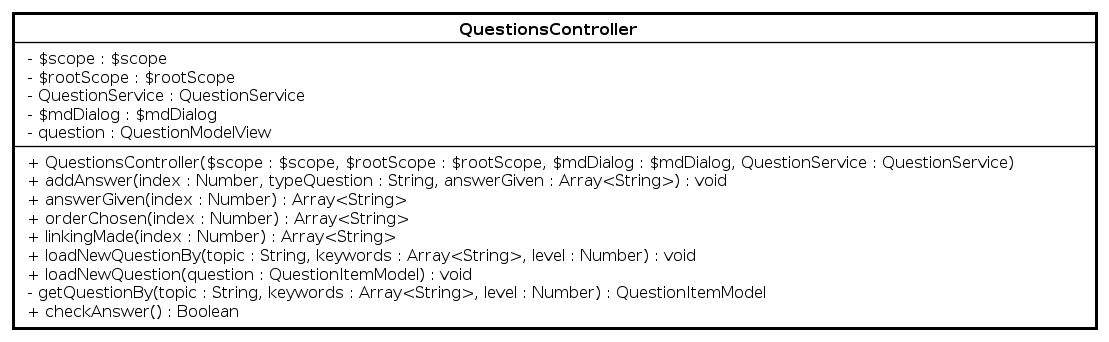
\includegraphics[scale=0.45]{UML/Classi/Front-End/QuizziPedia_Front-end_Controller_QuestionsController.png}
	\caption{QuizziPedia::Front-End::Controllers::QuestionsController}
\end{figure} \FloatBarrier
\begin{itemize}
	\item \textbf{Descrizione}: questa classe permette di gestire il recupero delle domande per poterle stampare nella modalità allenamento;
	\item \textbf{Utilizzo}: fornisce le funzionalità per il recupero delle domande esistenti nel database al fine di mostrarle durante la modalità allenamento nell'apposito template;
	\item \textbf{Relazione con altre classi}:
	\begin{itemize}
		\item \textit{IN} \texttt{HeaderTextQuestionDirective}: rappresenta il componente grafico che presenta all'utente il testo della domanda, l'argomento e le parole chiave. Viene gestito dinamicamente all'interno della view TrainingView attraverso il controller TrainingController; 
		\item \textit{IN} \texttt{TrueFalseAnswerDirective}: rappresenta il componente grafico che permette all'utente di visualizzare la domanda vero e falso. Viene gestito dinamicamente all'interno della view TrainingView attraverso il controller TrainingController; 
		\item \textit{IN} \texttt{MultipleChoiceAnswerDirective}: rappresenta il componente grafico che permette all'utente di visualizzare la domanda a risposta multipla. Viene gestito dinamicamente all'interno della view TrainingView attraverso il controller TrainingController; 
		\item \textit{IN} \texttt{LinkingAnswerDirective}: rappresenta il componente grafico che permette all'utente di visualizzare la domanda di collegamento. Viene gestito dinamicamente all'interno della view TrainingView attraverso il controller TrainingController; 
		\item \textit{IN} \texttt{SortImagesAnswerDirective}: rappresenta il componente grafico che permette all'utente di visualizzare la domanda ad ordinamento di immagini. Viene gestito dinamicamente all'interno della view TrainingView attraverso il controller TrainingController; 
		\item \textit{IN} \texttt{SortTextAnswerDirective}: rappresenta il componente grafico che permette all'utente di visualizzare la domanda ad ordinamento di stringhe. Viene gestito dinamicamente all'interno della view TrainingView attraverso il controller TrainingController; 
		\item \textit{IN} \texttt{EmptySpaceAnswerDirective}: rappresenta il componente grafico che permette all'utente di visualizzare l'esercizio a riempimento di spazi vuoti. Viene gestito dinamicamente all'interno della view TrainingView attraverso il controller TrainingController; 
		\item \textit{IN} \texttt{ClickableAnswerDirective}: rappresenta il componente grafico che permette all'utente di visualizzare la domanda ad area cliccabile nell'immagine. Viene gestito dinamicamente all'interno della view TrainingView attraverso il controller TrainingController;  
		\item \textit{IN} \texttt{QuestionServices}: questa classe permette di ottenere domande esistenti e salvare nuove domande;
		\item \textit{IN} \texttt{QuestionItemModel}: ;
		\item \textit{OUT} \texttt{FillingQuestionnaireController}: ;
		\item \textit{IN} \texttt{RightDirectiveModel}: ;		
	\end{itemize}
	\item \textbf{Attributi}:
	\begin{itemize}
		\item \texttt{-} \texttt{\$scope: \$scope} \\
		Campo dati contenente un riferimento all’oggetto \$scope creato da \textit{Angular\ped{G}}, viene utilizzato come mezzo di comunicazione tra il controller e la view. Contiene gli oggetti che definiscono il model dell’applicazione;
		\item \texttt{-} \texttt{\$rootScope: \$rootScope} \\
		Campo dati contenente il riferimento all'oggetto globale \$rootScope creato da \textit{Angular\ped{G}}. Viene utilizzato per rendere accessibile a tutti i controller e a tutte le view l'oggetto \texttt{QuestionItemModel}. In questo caso viene utilizzato per inserire in \$rootScope l'oggetto di ritorno della chiamata a \texttt{getQuestion} del service \texttt{QuestionsService};
		\item \texttt{-} \texttt{QuestionsService}: permette di ottenere domande esistenti tramite chiamata di metodo specifici;
	\end{itemize}
	\item \textbf{Metodi}:
	\begin{itemize}
		\item \texttt{+} \texttt{QuestionsController(\$scope: \$scope, \$rootscope: \$rootscope, QuestionService: QuestionService)}: \\ Metodo costruttore della classe. Cicla nell'oggetto QuestionItemModel ricevuto e si interfaccia con la view che andrà a recuperare e stampare la giusta direttiva della tipologia di domanda. \\
		\textbf{Parametri}:
		\begin{itemize}
			\item \texttt{-} \texttt{\$scope: \$scope} \\
			Campo dati contenente un riferimento all’oggetto \$scope creato da \textit{Angular\ped{G}}. Viene utilizzato come mezzo di comunicazione tra il controller e la view. Contiene gli oggetti che definiscono il viewmodel e il model dell’applicazione;
			\item \texttt{-} \texttt{\$rootScope: \$rootScope} \\
			Parametro contenente il riferimento all'oggetto globale \$rootScope creato da \textit{Angular\ped{G}}. Viene utilizzato per rendere accessibile a tutti i controller e a tutte le view l'oggetto \texttt{QuestionItemModel}. In questo caso viene utilizzato per inserire in \$rootScope l'oggetto di ritorno della chiamata a \texttt{getQuestion} del service \texttt{QuestionsService}; 
			\item \texttt{QuestionService: QuestionService} \\ Parametro che permette di ottenere domande esistenti tramite chiamata di metodo specifici;
		\end{itemize}
		\item \texttt{+} \texttt{getQuestion(): QuestionItemModel} \\ Metodo che richiede al back-end una domanda;
	\end{itemize}
\end{itemize}

